\chapter{Finanzen}
\label{chap:finanzen}

\section{Finanzierungskonzept}
Unser Unternehmen wird mit diesem Projekt gegr\"undet. Durch Crowdfunding kann man auf einfache Weise erfahren, ob ein Produkt f\"ur potentielle Kunden attraktiv ist oder nicht. Die Finanzierung des Projekts wird in diesem Fall durch Darlehen anstatt Eigenkapital gegr\"undet. Bei den meisten Crowdfundingplatformen muss man einen Kapitalbedarf angeben (auch Goal genannt), der die Realisierung des Projekts erm\"oglicht. Wenn der Kapitalbedarf innerhalb von 30 Tagen erreicht wird, kann das Unternehmen dieses Geld fordern und die Produktion des Produkts beginnen. Innerhalb von drei Jahren sollten dann alle Produkte geliefert werden. Das Unternehmen braucht momentan keine Werbung, weil die Kunden durch Crowdfunding gesucht werden.\\
Da das Unternehmen noch nicht existiert, mussten wir einige Werte absch\"atzen:\\
\begin{itemize}
\item \textbf{Anzahl Kunden:} Wir haben die Anzahl Kunden an der durchschnittlichen Anzahl Kunden von anderer \"ahnlichen Projekten abgesch\"atzt. Einige Projekte im IT Bereich erhalten bis zu 16000 Kunden (oder Backers). 
\item \textbf{Gewinn:} Wir m\"ochten einen Gewinn von 10000 Franken pro Jahr erreichen.
\item \textbf{Material und Produktion:} Wir haben die Materialkosten pro St\"uck bei Fr. 10.- gesch\"atzt, und die Produktionskosten (Strom, Verpackung, usw.) bei Fr. 2.- .
\end{itemize}

Erkl\"arung der \"ubrigen Kosten:\\
\begin{itemize}
\item \textbf{L\"ohne:} Unser Team besteht aus 6 Personen. \\
\begin{table}[H]
\centering
\caption{L\"ohne}
\label{L\"ohne}
\begin{tabular}{lll}
\textbf{Position} & \textbf{Monatsgehalt}  \\ \hline
  \textbf{CEO} &  Fr. 4700.- \\ \hline
 \textbf{CFO} &  Fr. 4700.- \\ \hline
 \textbf{Technischer Direktor}& Fr. 4700.-  \\ \hline
 \textbf{Mitarbeiter} &Fr.  3500.- \\ \hline
 \textbf{Durchschnitt} & Fr. 4000.-\\ \hline
\end{tabular}
\end{table}
\item \textbf{Webserver:} Um unser Produkt zu vermarkten und den Kontakt zu unseren Kunden zu pflegen.

\item \textbf{Crowdfunding Taxe:} Webseiten wie Kickstarter und Indiegogo verlangen einen Anteil von 10\% des Goals, wenn das Goal erreicht wird.
\item \textbf{Mietzins:} Fr. 700.- pro Monat
\item \textbf{Copyright:} Fr. 100.-
\item \textbf{Abschreibungen:} wir buchen Abschreibungen auf Produktionsmaschinen und sonstigem (Ankauf Fr. 5000.-), in der h\"ohe von 10\% pro Jahr (angenommene Lebensdauer: 10 Jahre).
\item \textbf{Analyse und Marketing:} Anfangsstudien die vor dem Crowdfunding gemacht wurden.
\end{itemize}
Da alle Teammitglieder Aktion\"are des Unternehmens sind, wird der Jahresgewinn auf alle Mitglieder verteilt.
\section{Steuern}
Unser Unternehmen wird seinen Sitz in Deisswil bei M\"unchenbuchsee haben. Die Steuern f\"ur einen Gewinn von Fr. 10000.- pro Jahr betragen Fr. 1300.- im Jahr.
\section{Zukunft}
Wir haben die Finanzplanung f\"ur die ersten 3 Jahre erstellt. Innerhalb dieser 3 Jahre werden wir den Backers das Produkt liefern. Falls die Nachfrage vorhanden ist, planen wir eine neue Version des Smoilet Produkts in den folgenden Jahren herzustellen. 
\section{Tabellen}
Die nachfolgenden Tabellen illustrieren die zu erwartenden variablen und fixen Kosten. Die Fixkosten nehmen im Verlauf der weiteren Jahre ab, da z.Bsp. die Analyse und Marketing Kosten nur im ersten Jahr anfallen.
\begin{figure}[H]
	\centering
		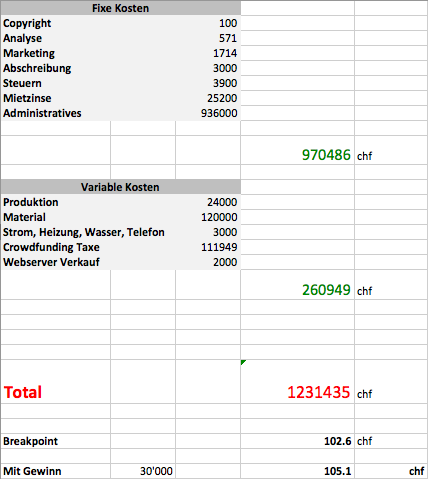
\includegraphics[scale=0.7]{bilder/3Jahre.png}
	\caption{Kosten\"ubersicht 3 Jahre}
	\label{fig:3Jahre}
\end{figure}
\begin{figure}[H]
	\centering
		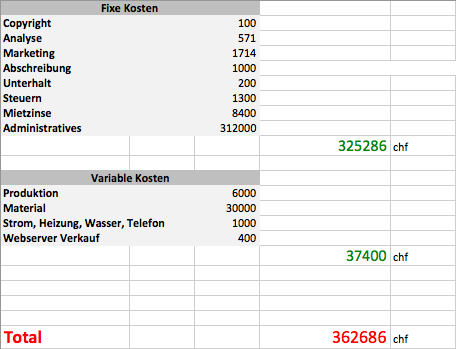
\includegraphics[scale=0.7]{bilder/Jahr1.png}
	\caption{Kosten\"ubersicht 1. Jahr}
	\label{fig:Jahr1}
\end{figure}
\begin{figure}[H]
	\centering
		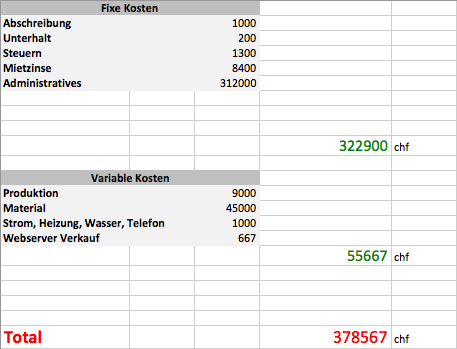
\includegraphics[scale=0.7]{bilder/Jahr2.png}
	\caption{Kosten\"ubersicht 2. Jahr}
	\label{fig:Jahr2}
\end{figure}
\begin{figure}[H]
	\centering
		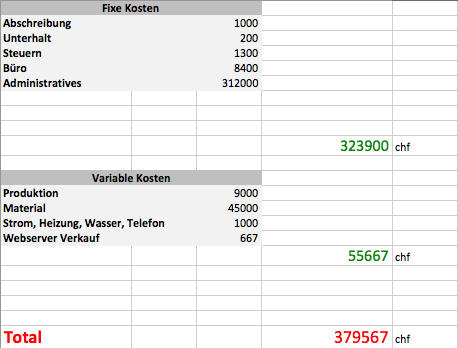
\includegraphics[scale=0.7]{bilder/Jahr3.png}
	\caption{Kosten\"ubersicht 3. Jahr}
	\label{fig:Jahr3}
\end{figure}
\begin{figure}[H]
	\centering
		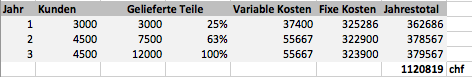
\includegraphics[scale=0.7]{bilder/kosten_ubersicht.png}
	\caption{Jahrestotal}
	\label{fig:Jahrestotal}
\end{figure}
\section{Kapitalbedarf}
\section{Fazit}
Um den Finanzteil mit einer realistischen Planerfolgsrechnung abzuschliessen, w\"aren wir auf genaue Angaben \"uber Kosten angewiesen. Leider ist es im Rahmen dieser Arbeit nahezu unm\"oglich, an diese Zahlen zu gelangen. Ziel des Crowdfundings liegt nicht prim\"ar in der Umsatzsteigerung, sondern in der Gewinnmaximierung durch Kostenersparnisse in Bezug auf Werbung und Kundensuche. 